In this section, we introduce our strategy in SMTLe that can exploit the knowledge from different types of classifiers. In general, for each example in the target domain, we use its output class probabilities from the source models as the auxiliary bias term to adjust the final output.

%\subsection{Auxiliary Bias from the source model}
To make our method compatible with different types of source model, we have to find a solution to align the knowledge of different types of classifier. It is clear that most of the existing classifiers can output the class probability for the input examples. Therefore, in SMTLe, we use the class probability of the target examples from the source model to align the knowledge of the different types of source model.  

To use the aligned source knowledge, we use a straight-forward way, by using the class probability as the auxiliary information to adjust the output of the target model (see Figure \ref{fig:ab}).
However, as we know that due to the domain shift, the performances of the different source models vary on the target domain. Therefore, to compensate this domain shift, we apply different weights to different source model outputs. Here, the weight of each model reflects the relatedness between the source model and the target domain. The more related they are, the larger weight we should apply. Specifically, in this paper, we call it \textit{transfer parameter}. Therefore, for any target learning $D_T=\{x,y\}$ and the given source model $f'$, our goal is to find the target model $f$:
\begin{equation}\label{eq:low_opt}
f=\underset{f \in \mathcal{F}}{\arg \min}\ell\left(f+\beta f',D_T\right)
\end{equation} 
where $\beta$ is the transfer parameter and $\ell(\cdot,\cdot)$ is the loss function to learn the target model.

\begin{figure}\label{fig:ab}
	\centering
	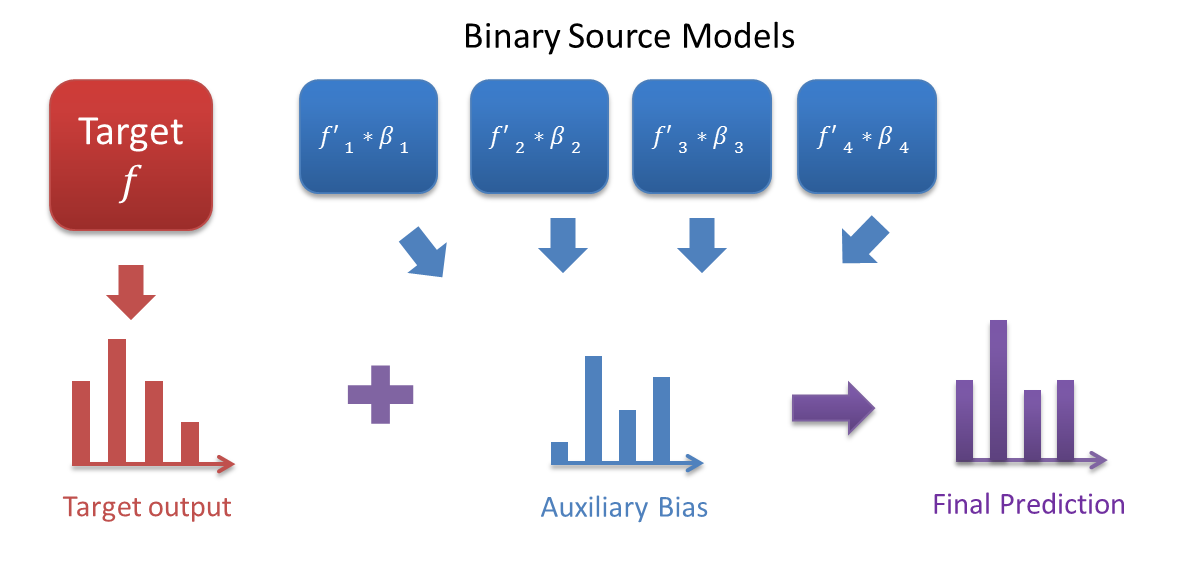
\includegraphics[scale=0.6]{fig/ab.png}
	\caption{Demonstration of using the source class probability as the auxiliary bias to adjust the output of the target model.}
\end{figure}
%Actually, using the output of the classification model as the auxiliary information to train another model has been widely used in different learning scenarios. In Vapnik's \textit{Teacher-student} diagram, it is represented as the \textit{privileged knowledge} and in Hinton's \textit{Distillation} diagram \cite{hinton2015distilling}, it is called \textit{soft-labels}.
%Different from those previous works where the model used to general the auxiliary features is trained from the same domain, our model is trained from a different but related domain.

There are several advantages of our feature augmentation with class probability: (1) It is an effective and easy way to align the knowledge from different types of source model.
(2) Features are naturally normalized in the same dimension as the class probability is always in the interval $[0,1]$. (3) The bonus advantage: increase the selection of the source domain. As SMTLe can select more types of source model, we have more options to select our source domain. As long as the model has the knowledge of the class we want (even though we may only need knowledge of one class in a multi-class classifier), we can still exploit the knowledge.

From Eq. \eqref{eq:low_opt} we can see that, once we can determine the value of the transfer parameter $\beta$, we are able to find the target model $f_T$. In the next part, we will show how we can effective estimate the unbiased transfer parameter effectively.





